% Template for NIME 2017
%
% Modified by Cumhur Erkut on <2016-10-11 Tue>
% Modified by Edgar Berdahl on 5 November 2014
% Modified by Baptiste Caramiaux on 25 November 2013
% Modified by Kyogu Lee on 7 October 2012
% Modified by Georg Essl on 7 November 2011
%
% Based on "sig-alternate.tex" V1.9 April 2009
% This file should be compiled with "nime-alternate.cls"


\documentclass{nime-alternate}
\usepackage[utf8x]{inputenc}
\PrerenderUnicode{aâîțșĂÎÂȚȘ}
%\usepackage{dirtytalk}

\begin{document}
%
% --- Author Metadata here ---
\conferenceinfo{NIME'17,}{May 15-19, 2017, Aalborg University Copenhagen, Denmark.}

\title{SoundThimble: A High Resolution Real-Time\\Gesture Sonification Framework}

%
% You need the command \numberofauthors to handle the 'placement
% and alignment' of the authors beneath the title.
%
% For aesthetic reasons, we recommend 'three authors at a time'
% i.e. three 'name/affiliation blocks' be placed beneath the title.
%
% NOTE: You are NOT restricted in how many 'rows' of
% "name/affiliations" may appear. We just ask that you restrict
% the number of 'columns' to three.
%
% Because of the available 'opening page real-estate'
% we ask you to refrain from putting more than six authors
% (two rows with three columns) beneath the article title.
% More than six makes the first-page appear very cluttered indeed.
%
% Use the \alignauthor commands to handle the names
% and affiliations for an 'aesthetic maximum' of six authors.
% Add names, affiliations, addresses for
% the seventh etc. author(s) as the argument for the
% \additionalauthors command.
% These 'additional authors' will be output/set for you
% without further effort on your part as the last section in
% the body of your article BEFORE References or any Appendices.

\numberofauthors{4}
%
\author{
% You can go ahead and credit any number of authors here,
% e.g. one 'row of three' or two rows (consisting of one row of three
% and a second row of one, two or three).
%
% The command \alignauthor (no curly braces needed) should
% precede each author name, affiliation/snail-mail address and
% e-mail address. Additionally, tag each line of
% affiliation/address with \affaddr, and tag the
% e-mail address with \email.
%
% 1st. author
\alignauthor
Ben Trovato\\
       \affaddr{Authors hidden for review}\\
       \affaddr{1932 Wallamaloo Lane}\\
       \affaddr{Wallamaloo, New Zealand}\\
       \email{trovato@corporation.com}
% 2nd. author
\alignauthor
G.K.M. Tobin\\
       \affaddr{Authors hidden for review}\\
       \affaddr{P.O. Box 1212}\\
       \affaddr{Dublin, Ohio 43017-6221}\\
       \email{webmaster@marysville-ohio.com}
%\and
% 3rd. author
%\alignauthor Grigore Burloiu\\
%       \affaddr{CINETic}\\
%       \affaddr{UNATC "I.L. Caragiale"}\\
%       \affaddr{Bucharest, Romania}\\
%       \email{gburloiu@gmail.com}
% 4th. author
%\alignauthor Bogdan Golumbeanu\\
%\affaddr{CINETic}\\
%\affaddr{UNATC "I.L. Caragiale"}\\
%\affaddr{Bucharest, Romania}\\
%\email{bogdangolumbeanu@yahoo.com}
}
% There's nothing stopping you putting the seventh, eighth, etc.
% author on the opening page (as the 'third row') but we ask,
% for aesthetic reasons that you place these 'additional authors'
% in the \additional authors block, viz.
%\additionalauthors{Additional authors: John Smith (The Th{\o}rv{\"a}ld Group,
%email: {\texttt{jsmith@affiliation.org}}) and Julius P.~Kumquat
%(K. Consortium, email: {\texttt{jpkumquat@consortium.net}}).}
\date{24 Jan 2017}
% Just remember to make sure that the TOTAL number of authors
% is the number that will appear on the first page PLUS the
% number that will appear in the \additionalauthors section.

\maketitle
\begin{abstract}
	
	
%\textit{SoundThimble} is an interactive installation, inspired by the game called Hunt the Thimble in which someone hides an object then guides the other players to its location by stating whether their position is “hot” – closer to the object, or “cold” – farther from the object. 

We introduce \textit{SoundThimble}, a platform for sonic interaction based on the relationship between human motion and virtual objects in 3D space.

The installation employs a Vicon motion capture system and custom software to track, interpret and sonify the movement and gestures of a performer in 3D space.
 
We distinguish between three interaction scenarios, centred around object searching, manipulation and arrangement. We illustrate the resulting extended possibilities of perception and expression via two case studies: a participative installation and a dance performance.

The software developed is open source and portable to similar hardware systems, leaving room for further extension of the installation mechanics.
\end{abstract}

\keywords{Sonification, motion capture, gesture spotting, interactive installation, synthesis}

\acmclassification1998{
\begin{itemize}
	\setlength\itemsep{-0.2em}
	\item Applied computing~$\rightarrow$~Sound and music computing
	\item Computing methodologies~$\rightarrow$~Motion capture
	\item Human-centered computing~$\rightarrow$~Gestural input
	\item Human-centered computing~$\rightarrow$~Auditory feedback
\end{itemize}

}

 
% \ccsdesc[500]{Computing methodologies~Motion capture}
% \ccsdesc[500]{Applied computing~Sound and music computing}
% \ccsdesc[300]{Human-centered computing~Auditory feedback}
% \ccsdesc[300]{Human-centered computing~Gestural input}

\section{Introduction}

%- motivation

%- challenges

%\textbf{- the Vicon system}\\ \par


High resolution three-dimensional motion tracking is traditionally used for animation in film and games, as well as for life sciences research and engineering applications~\cite{welch2002motion}. This technology has long been mined by the NIME community~\cite{dobrian2003gestural, nymoen2011soundsaber}, although in many early cases, technical limitations meant that the motion data transmission and the sound generation processes were not simultaneous~\cite{dobrian2003gestural, kapur2005framework}.


The \textit{SoundThimble} project harnesses current motion capture technology and gesture detection algorithms to develop new modes of sound exploration in an interactive installation context. Our aim is to push beyond the standard paradigms of isolated body motion audification~\cite{dobrian2003gestural,kapur2005framework} or sound control interfaces~\cite{eckel2009motion,nymoen2011soundsaber}, towards deeper narrative structures coupled with layered arrangement of music patterns.


Our implementation uses a state-of-the-art Vicon motion capture system\footnote{See  \url{https://www.vicon.com}.} containing eight Vantage 5-megapixel infrared cameras and two Bonita video cameras. Since the open-source software developed in this project\footnote{Available at  \url{https://github.com/RVirmoors/viconOSC}.} is\linebreak built around Vicon's Datastream SDK,\footnote{See  \url{https://www.vicon.com/products/software/datastream-sdk}.} the platform can be ported to both older and future Vicon-based systems.

In the remainder of the paper, we review relevant existing projects and technology (section~\ref{sec:related}), we describe the \textit{SoundThimble} concept and development (section~\ref{sec:proj}), we propose two applied case studies (section~\ref{sec:case}), and we conclude with a survey of remaining challenges and future perspectives (section~\ref{sec:conc}).


\section{State of the Art}
\label{sec:related}


Sonification, as the auditory representation of a datastream, has been a rich tool for the interpretation of human movement~\cite{hermann2011sonification}. From the musical perspective, infrared motion capture systems have been revealed as a powerful for expressive interaction in a controlled environment, with many of the results being translatable to more portable technologies~\cite{skogstad2010using,vigliensoni2012quantitative}.

In particular, Vicon motion capture systems have been used for over a decade for music applications~\cite{dobrian2003gestural,kapur2005framework,eckel2009motion,vigliensoni2012quantitative}. An software bridge for streaming OSC data from Vicon has been developed\footnote{See \url{http://sonenvir.at/downloads/qvicon2osc/}.}~\cite{eckel2009motion} as part of a concluded project, which proved to be incompatible with our current setup.

The current decade has seen qualitative advances in the interaction between human gesture and sound behaviour, made possible by real-time gesture recognition and following tools~\cite{probabilisticmodels}. These allow for more complex scenarios to be designed, where movement is used both for direct sonification and for multi-level control of system behaviour---features which our project channels into a coherent framework.

%GRIG: as scoate referinta asta, prea generic
%~\cite{Gestureanalysis}. ... .

\section{Project Description}
\label{sec:proj}

\subsection{Concept}

% inovare = abordarea spatializarii obiectelor sonore / acusmatics

The sound-thimble, as the basic building block of our framework, is based on the concept of \textit{sound object} in the Schaefferian sense, as a clearly delimited sounding unit, open to manipulation, arrangement and composition~\cite{schaeffer1998solfege}.

Such an entity, once instanced, can retain an ambiguous nature (spatially and acousmatically) or can switch to a more material state (positioned in space and tied to a causal source)~\cite{soundunseen}. The duality between the latent positioning of the object (which can be inferred from phenomena other than spatial sound reproduction), and the active sound spatialisation, once tied to motion data, becomes an innovative tool for sonic arts through sound sketching, auditory games and other realtime interaction scenarios.

\subsubsection{Interaction scenario}

\textit{SoundThimble} can be viewed as both an interactive sound installation and an auditory game, comprising three phases: search, manipulation, arrangement.


The game's narrative starts with a human player attempting to find a sound-thimble (a stationary virtual object, randomly positioned in 3D space), by analysing cues that are constantly shifting in the sonic fabric based on the human's movement relative to the object. Analogously to the traditional game of \textit{Hunt the Thimble} (a.k.a \textit{Hot or Cold}), the space between the human and the virtual object is correlated to sound synthesis and modulation parameters. Briefly, the closer one comes to the object, the more coherent the sound and vice-versa. 

Once the object is found, its sonic manifestation gains a richer causal relationship to the human: the player becomes a performer, and is now able to explore the object's sonic palette, and record a number of gestures that can be re-performed later, re-called, and used to trigger or manipulate sonic shifts and events.

Finally, the performer can drop the virtual object to the floor, or discard it by ``pushing" it outside of the installation boundaries. This triggers a new object to be randomly generated, while the player retains a degree of control over the initial object via the recorded gestures. Both objects are now in a latent state, with the new one guiding the player's search, and the previous one responding to the learned set of gestures.

This repeating scenario is outlined in Figure~\ref{fig:concept}: objects are randomly generated, the performer finds them, defines gestures and interacts sonically with them before arranging them in a pleasing configuration. With each spawning of a new object or assignment of a new gesture, the game becomes more challenging and complex, but also more flexible and rewarding.


\begin{figure}[t]
	\centering
	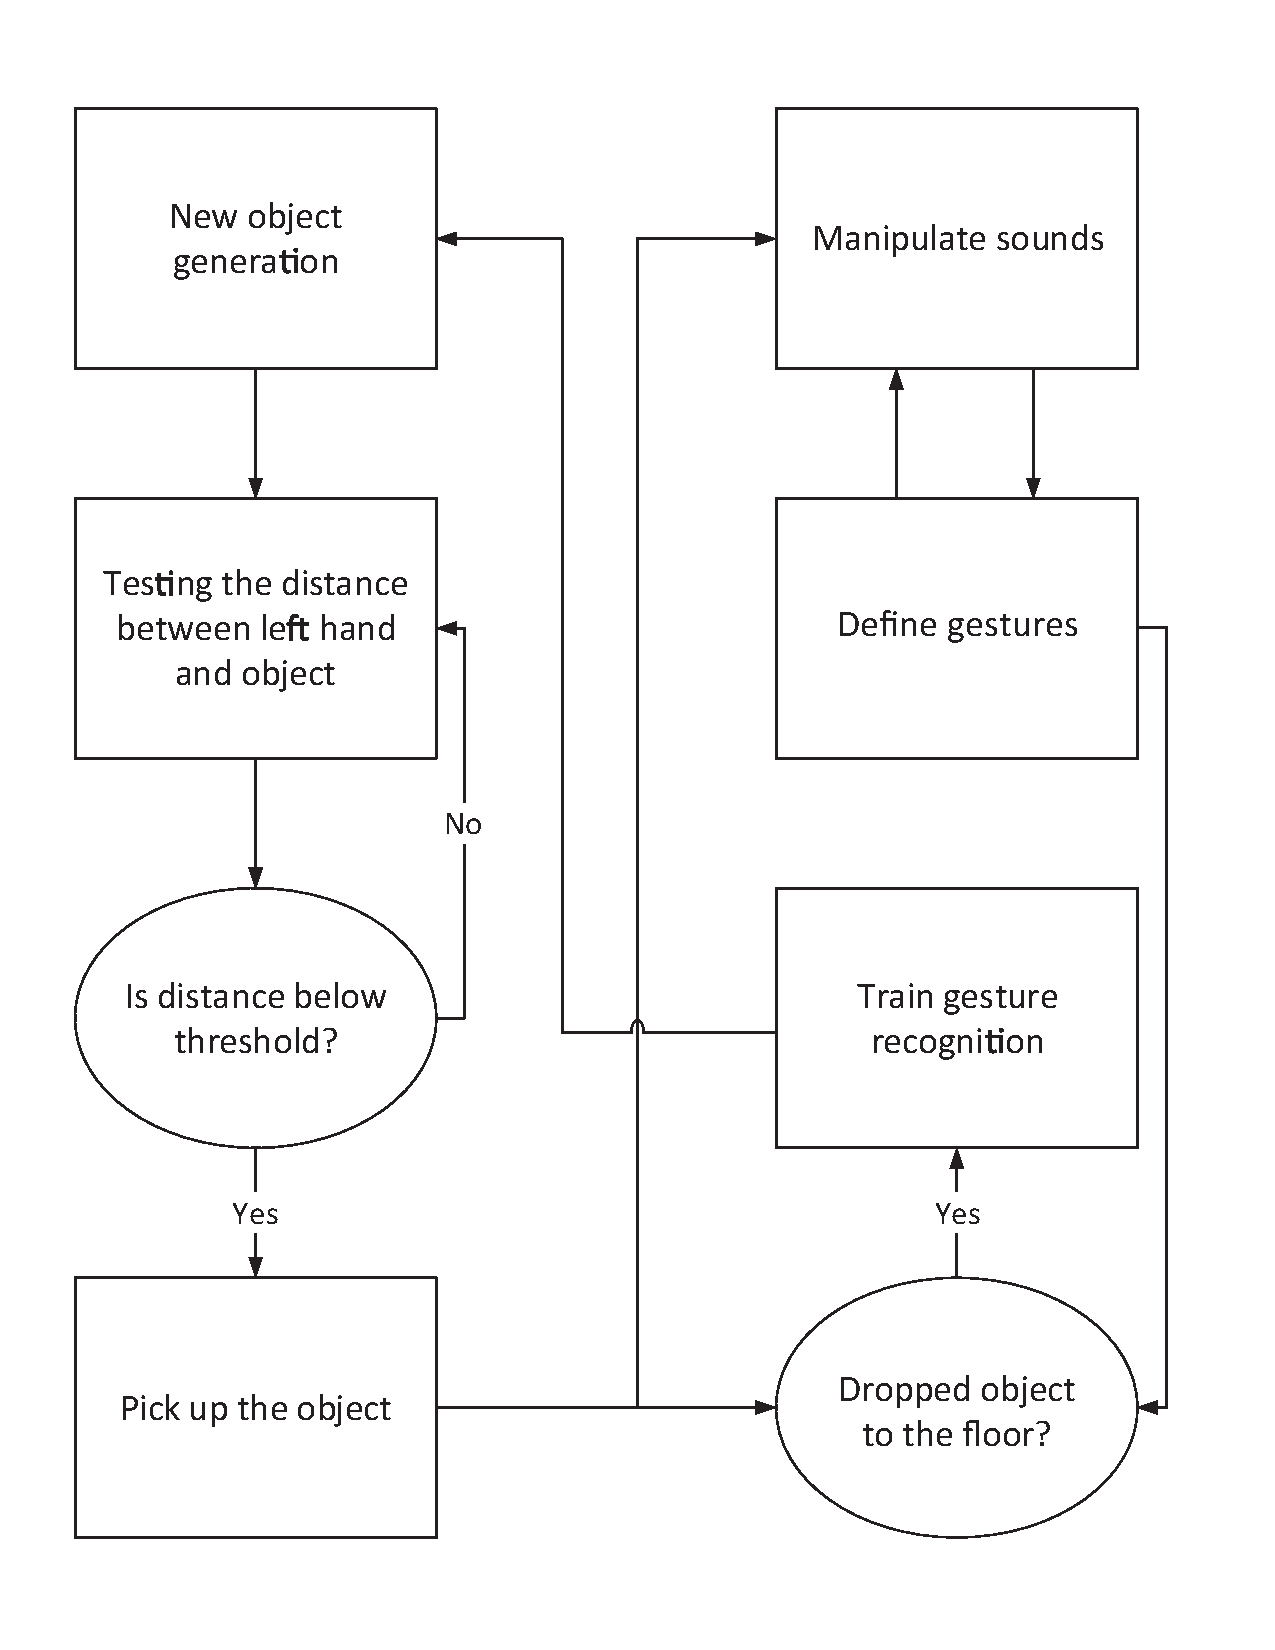
\includegraphics[width=.65\columnwidth]{img/concept}
	\caption{\textit{SoundThimble} interaction workflow.}
	\label{fig:concept}
\end{figure}

\subsubsection{Performance aesthetic}

- text Bogdan

Our present approach is informed by Worrall's study~\cite{worrall2013understanding}, which reveals a necessity for the mapping of minute gestural inflections to alter sonic material with a view to certain modes of listening. The aim of \textit{SoundThimble} is to fluctuate between: reflexive, kinaesthetic, connotative, empathetic, reduced.

\subsection{Implementation}

%Many interactions and programable elements which are included in the concept have an exactly function and usefulness. These elements are created in MAX with the help of Vicon SDK and OSC C++ library. The concept suppose an interactive action of a performer or a simple user with an virtual object which has associated gestures defined by person. Virtual object interaction acts in sound design utility like a master controller. Searching for a certain object comes with an audio feedback which makes the search easier.  A dynamic mapping of marker's coordinates is necessary to transfer data between Nexus and MAX.

%One of the first challenges was to create a method of sending real-time from Vicon to MaxMSP where data would be processed and used to generate and manipulate sound. By default, the Vicon system does not support the Open Sound Control (OSC) protocol (ref), needed to communicate with MaxMSP. To overcome this limitation, some code modifications and additions have been implemented inside Vicon’s Blade sdk.

\begin{figure}[t]
	\centering
	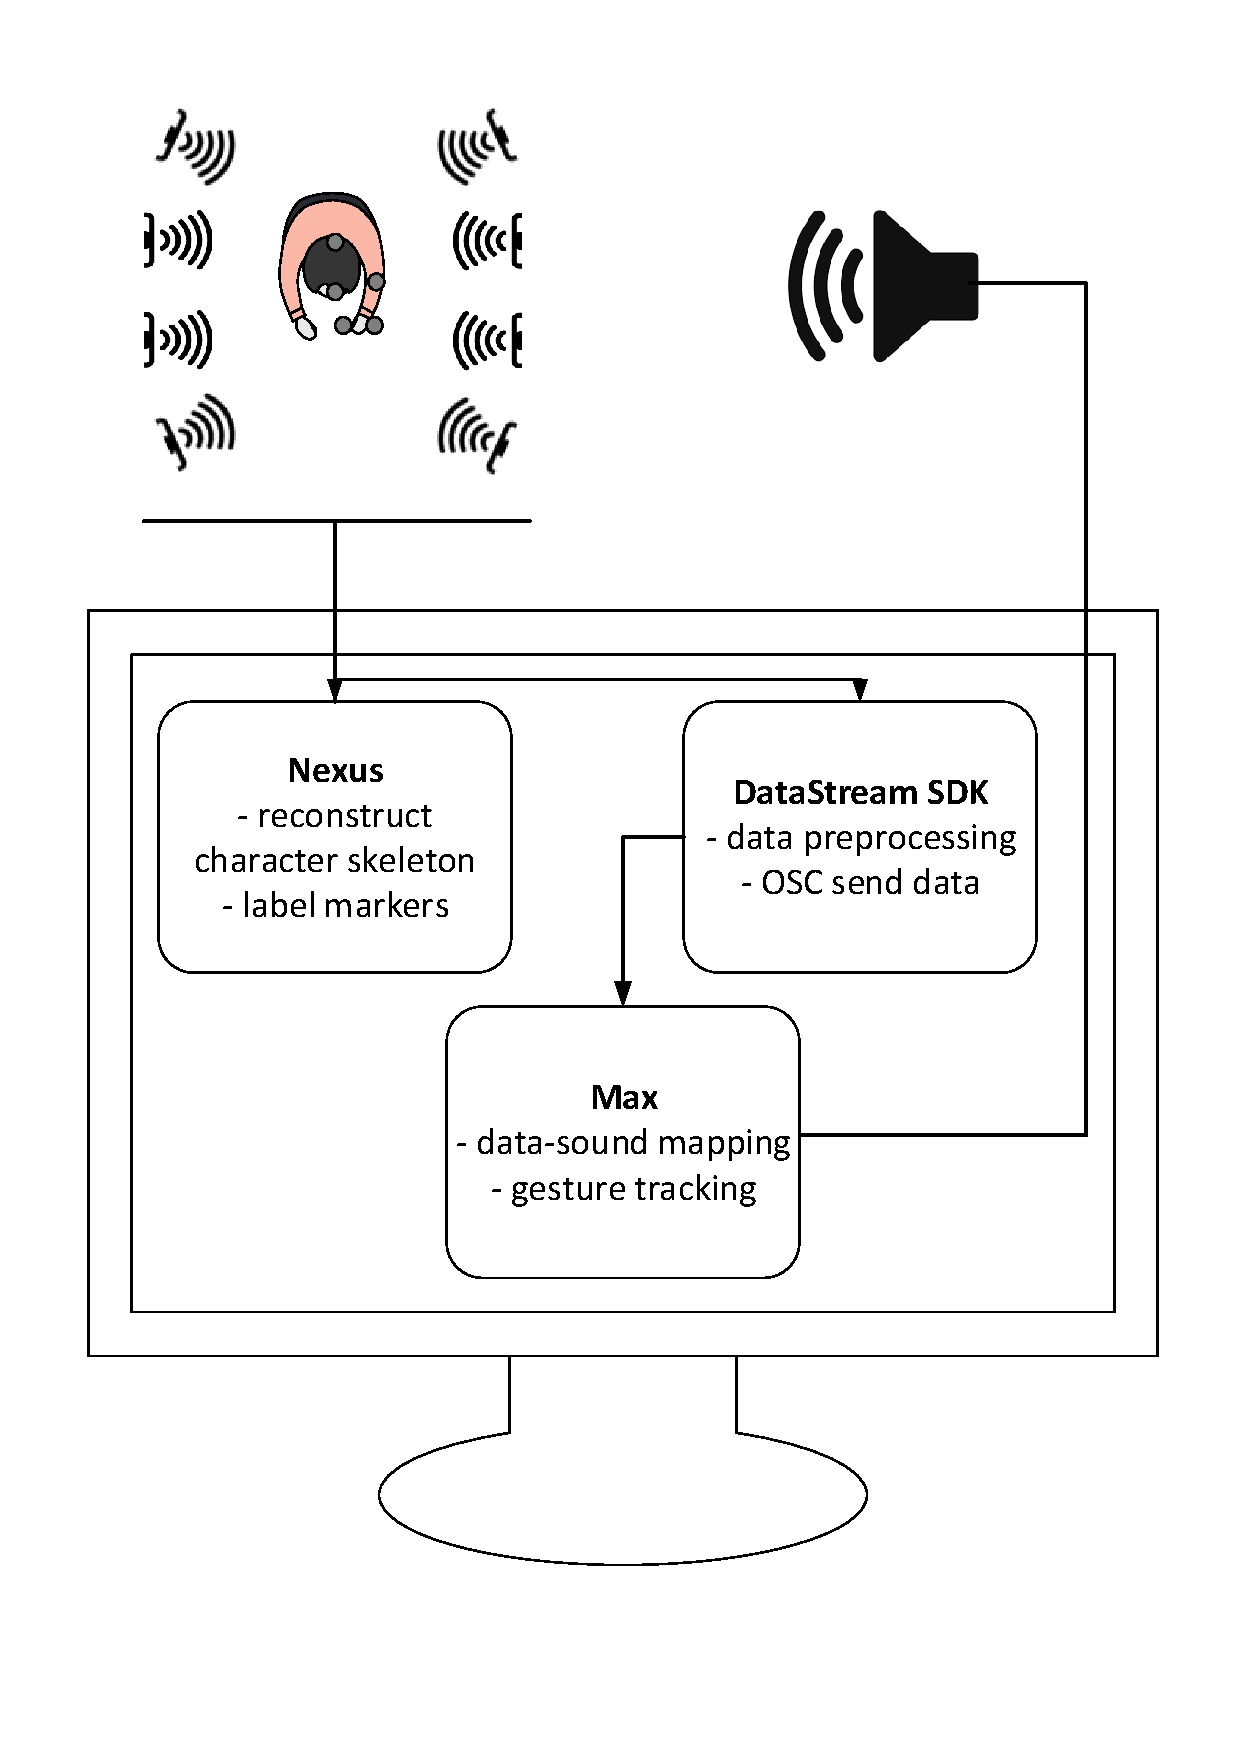
\includegraphics[width=.65\columnwidth]{img/archi}
	\caption{\textit{SoundThimble} framework architecture.}
	\label{fig:archi}
\end{figure}

The framework architecture diagram is laid out in Figure~\ref{fig:archi}. Three-dimensional sensor data is streamed into the Vicon Nexus software, which is able to reconstruct and label the underlying character skeleton. The gesture recognition and sonification algorithms are programmed in Max\footnote{Max is a state-of-the-art programming environment for realtime multimedia performance: \url{http://cycling74.com/}.}, which generally receives control data via the OSC\footnote{OpenSoundControl is a multimedia communication protocol: \url{http://opensoundcontrol.org/}.} protocol. Since Vicon systems do not support OSC out of the box, we used the \textit{oscpack}\footnote{See \url{http://www.rossbencina.com/code/oscpack}.} library to extend the DataStream C++ SDK and send OSC bundles to Max.


\subsubsection{Character design}

Figure~\ref{fig:nexus} shows a skeletal reconstruction in the Nexus environment. Since our project is intended as a public installation, we pursued a minimal amount of markers, for ease of setup and prototyping. The resulting configuration---sufficient for tracking hand and arm gestures, while ensuring the redundancy needed when one marker is obscured from the cameras---consists in 5 markers: two positioned on the head, one on the forearm, and two on the hand (thumb and index finger).

\begin{figure}[ht]
	\centering
	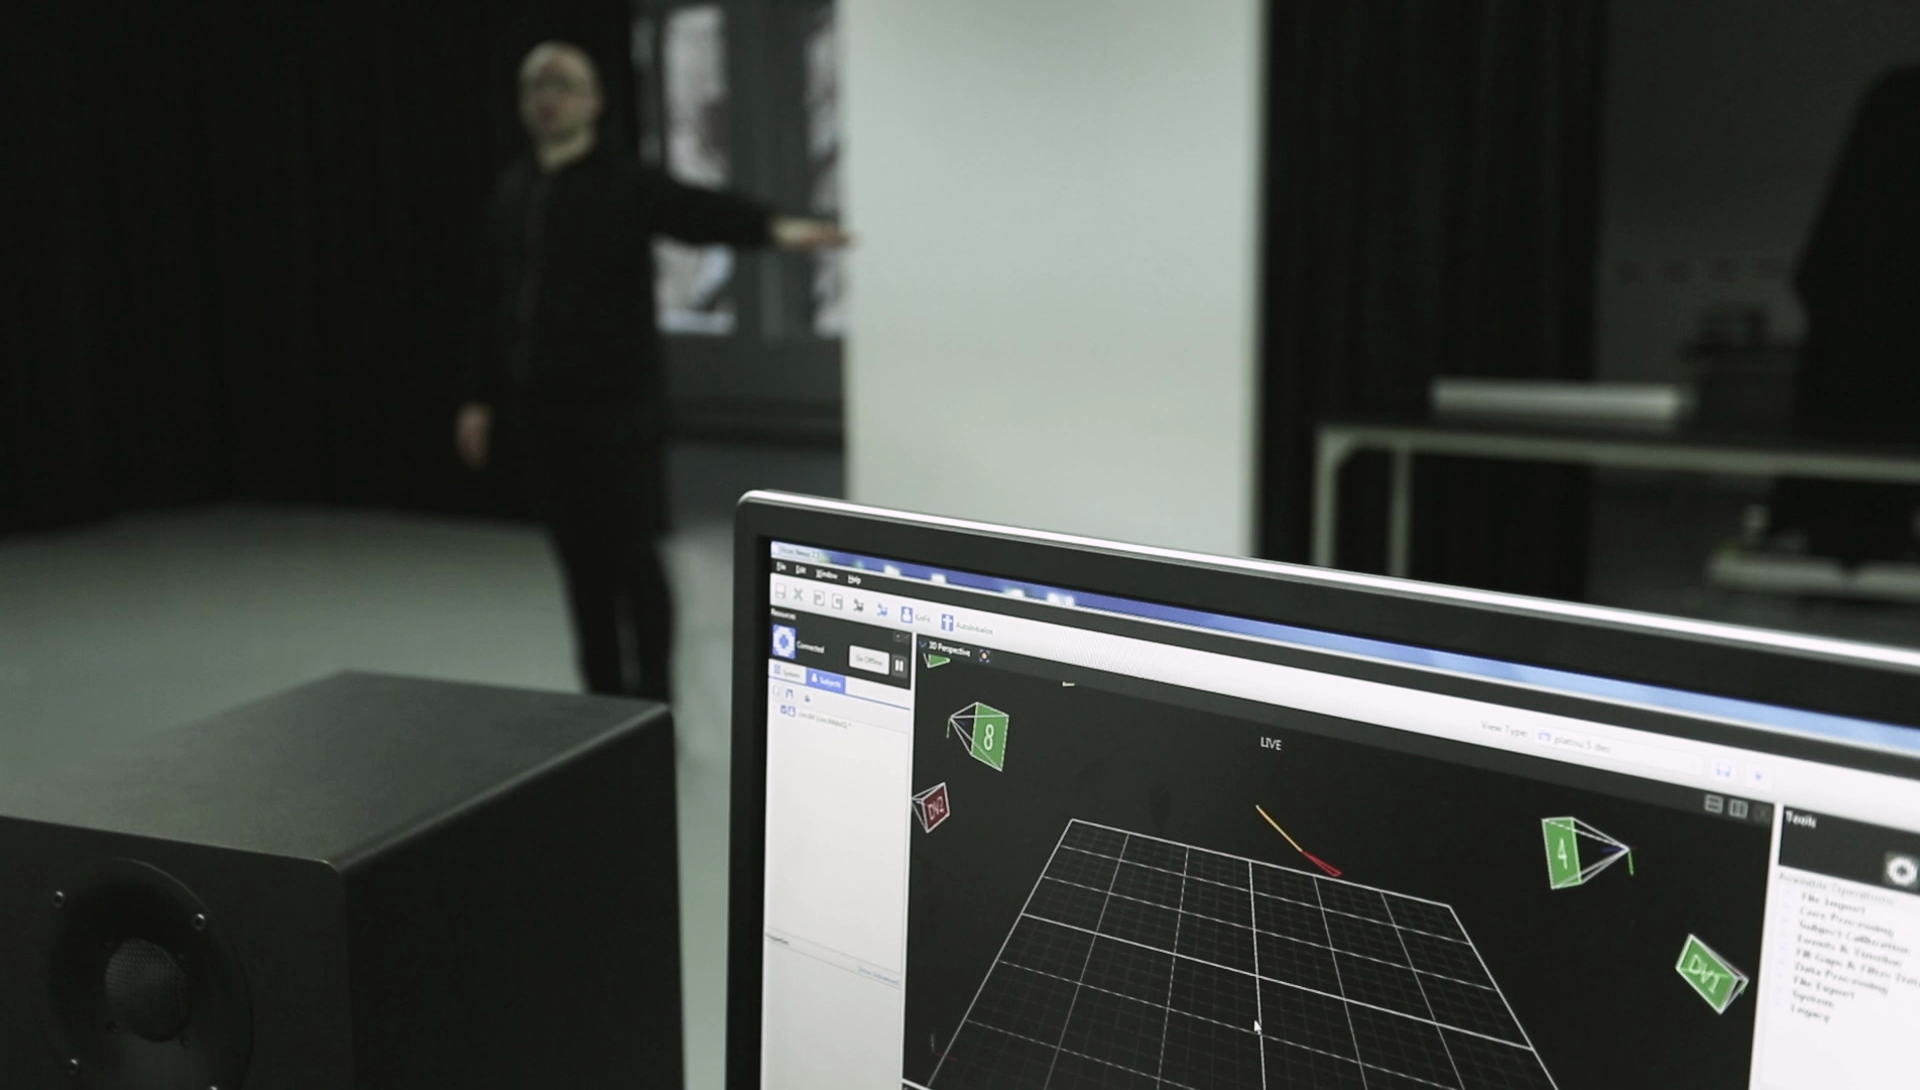
\includegraphics[width=\columnwidth, clip, trim={12cm 0 0 0}]{img/nexus}
	\caption{A performer tracked in Vicon Nexus. Two visible segments: head-forearm, forearm-hand.}
	\label{fig:nexus}
\end{figure}

Each OSC bundle sent through the SDK consists of the following:
\begin{itemize}
	\item 3D coordinates for the head (averaged from the two head markers);
	\item 3D coordinates for the hand (averaged from the two hand markers);
	\item distance between thumb and index finger.
\end{itemize}

All three items are sent only if non-zero, i.e. for the head and hand coordinates at least one of the respective markers is active, while for the distance computation, both markers need to be visible and correctly labelled. The forearm marker is used only for segment reconstruction, and is not sent via OSC.

%Implementation of the concept presented above requires Nexus, Vicon SDK and MAX sotware. Every character involved in the scene is defined by a limited number of markers. In this case, two markers are positioned on the head, one marker is positioned on elbow and the others 2 on the hand (thumb and index finger). Every marker has associated a name in Nexus and between them 6 segments are drawn. It is very important in realtime capture motion, that the marker to have assigned correct coordinates.

%Also, the Vicon DataStream Software Development Kit (SDK) admits inside changes such as labeling markers, timecode generation and framerate.

The described configuration produces highly stable and responsive inputs into the Max system, with a spatial resolution of 1mm and a latency of 5ms at a frame rate of 500hz.\cite{song2016fast}
Bonita sub sample ratio 5:1 = 500

\subsubsection{Object generation \& interaction mechanics}
%GRIG: nu e cazul sa prezentam Max pe larg aici. Eventual o propozitie scurta mai sus...
%Max is a realtime visual programing environment for music and multimedia arts that helps you build stand-alone applications, plugins and mixing audio signals. In order to create interactive sounds, attractive grapichs and special effects, MAX creates a connection between virtual objects and subpatches\footnote{See \url{http://www.cycling74.com/}.}.
%Manipulating objects algorithm consists of some major steps: object generation, finding the object, picking up the object, dropping the object to the floor.

The following object-related mechanics are implemented as basic algorithms in Max: generation, detection, dropping.

Object generation is executed randomly within the boundaries of the motion capture field, as defined in the Vicon calibration phase. Detection of the sound-thimble occurs when the distance between hand and object falls below a set threshold. By default this threshold is set at 200mm radial distance; lowering it can make the game considerably more difficult. Once the object is detected, it becomes mobile, its coordinates tracking those of the hand's.

Finally, a simple thresholding of the $z$-axis (height) value of the hand position serves to put down the object. If the velocity computed on the $x$ or $y$ axes (horizontal plane) is high enough, then the object is pushed in the respective direction, and is able to leave the area of the installation, essentially being removed from the game.
At this point, a new object is introduced. The system keeps track of all object coordinates, as they appear and disappear over time.

 %According to this, a performer can handle as many objects as he wants.


\subsubsection{Gesture recognition}

We use the thumb-index finger distance value to enable gesture recording while the two fingers are kept close together. The input data captured into \textit{MuBu} multi-buffer containers~\cite{mubu} consists of pairs of values:
\begin{itemize}
	\item $\sqrt{\frac{(\Delta x)^2 + (\Delta y)^2}{2}}$;
	\item $\Delta z$,
\end{itemize}
where $\Delta x$, $\Delta y$, $\Delta z$ are the respective differences between head and hand coordinates. This feature preprocessing serves two purposes:

Firstly, gestures are recorded based on the position of the hand relative to the head, thus becoming invariable to the performer's absolute \textit{position} within the space. Secondly, by composing the $x$ and $y$ values into a single feature, gestures become invariable to the performer's \textit{orientation} on the horizontal plane. Thus, gestures can be recorded and recalled anywhere within the space, irrespective of the direction the performer is facing.

The input features are fed to one of two gesture recognition algorithms, both part of the \textit{MuBu} package. The first, based on Hierarchical Hidden Markov Models (HHMM), is implemented in the \texttt{mubu.hhmm} Max object. HHMMs are a generalization of HMM where each state is considered to be a self-contained probabilistic model~\cite{probabilisticmodels,hhmm}. The second is the \textit{Gesture Follower} \texttt{gf} Max object, based on a Sequential Monte Carlo inference engine~\cite{caramiaux2015adaptive}. 

The first method allows for \textit{gesture spotting}, i.e. it constantly produces likelihood values of a certain gesture being active, together with an approximation of its completion rate. If these are over a certain threshold, the respective gesture is triggered. The second method is more flexible and precise: the detected gesture can be followed at a variable rate or scale, even backwards. The only drawback is that it requires a start trigger, which we send by quickly attaching and separating the thumb and index finger.

Each generated object has a number of gestures associated to it. When an object is dropped to the floor, the classifier is (re)trained with the new data, and consequently gestures can act as on/off switches for a particular sonic behaviour (if they are performed/spotted once at a time), or as continuous controllers (if they are repeated). When several objects exist on the floor, one specific movement might act on one or more objects, depending on which detection likelihoods exceed the threshold. 

%In order to control every generated object, there are associated 2 or 3 gestures saved by the performer, but there is a limited time for the gestures to be executed. Predefined gestures offer the possibility to delete the gesture just saved and also indicate the moment the gesture is recorded.

\subsubsection{Sound design}


Each sound-thimble has a corresponding sound design patch, differing in (a) the source sound material used, (b) the synthesis techniques applied, and/or (c) the control mapping schema to the object search and manipulation variables. The various combinations of (a), (b) and (c) give rise to a growing library of objects, each with its own character. By designing various interaction rules for each object, segments are linked to different synthesis parameters or groups of parameters resulting in a continuously evolving, organic soundscape.

We differentiate between the three phases of the installation in terms of mapping technique and level of sonic interactivity. The search mode employs straightforward parameter mapping, where human-object distance measures are linked to synthesis parameters, while the manipulation phase relies on a model-based mapping approach where different gestures and actions reach deeper levels of control~\cite{hermann2011sonification}. Finally, variations on both these techniques occur in the arrangement phase.


The synthesis patches used for search are built around a process of decorrelation~\cite{101}: the farther the human's hand from the object the more decorrelation occurs, up to the point where each instance of the signal becomes a distinct sonic entity. This is done by continuously modulating each of the copies in terms of pitch (FM) and amplitude (AM) with low frequency oscillators (LFO’s). Changes in frequency, amplitude and wave shape of the LFO’s lead to complex sonorities ranging from regular streams of sound to distinct iterations with a high degree of randomness. %By moving and assessing sonic shifts and the level of decorrelation, the performer is able to intuitively find the object. 
This mechanism is subtly mixed with a granular engine in a latent state, which gains more prominence in the manipulation phase.

In this mode, the 3D space is split into chunks, each one acting as a zone with its own mappings and interaction laws. The synthesis patches are based on the segmentation of a source sound into short grains. We built a granular synth with these controllable parameters: grain size, grain position, envelope shape, level of scattering, pitch, timbre and stereo width. Another patch implements a concatenative synth that traverses the grains guided by movement velocity and trajectory. Certain gestures trigger sonic events while interpolating between sets of parameter values via a convergent-mapping scheme~\cite{102}. %This patch is active in both the object search and manipulation phases, differing between them in the dimensionality of control and presence in the auditory scene. 
%In order for the user-experience to be truly engaging, a great deal of calibration needs to be done in respect to the physical space. This is done by setting and tweaking ranges, scaling laws, assigning thresholds and designing various function curves.


In the search phase, all sound design is based on two channels that can either be routed to multiple pairs of speakers or downmixed to mono and diffused on an arbitrary number of speakers. In the manipulation phase, the soundscape is spatialised to track the position of the performer. In the arrangement phase, the dropped object retains a ``root" source location, which can relate dynamically to the performer position when a gesture is executed: for instance, the granular patch sends spatialised grains back and forth between the dropped object and the performer.


In developing the sound design algorithms, we used two input data sources. The first one is motion capture data recorded in Nexus and played back through the SDK. For more flexibility and immediate control, we also developed a basic visual interface to monitor the input data and to manipulate it in virtual 3D space using the mouse, for instant auditory feedback. This feature comes in useful when specific motion data is not available and needs to be roughly simulated.

\section{Case studies}
\label{sec:case}

We present two applications of our platform: a participative installation, and a performance piece. They represent two manifestations of the \textit{SoundThimble} concept and infrastructure, through a pair of experiences: (1) the direct interaction with sound in space, and (2) the mediated interaction with sound and space of an audience member. In both cases, the range of sense and perception is extended through new experiences.


\subsection{Interactive installation}

- interaction analysis: Bogdan

\subsection{Dance performance}

The following is a sketch for a work currently under development. A performer enters the motion capture space, and commences a series of improvised motions, silently establishing the action space.

Once a threshold is reached, a virtual object is generated and the movement is no longer completely free, its range of action being directed by the relationship to the object position. Searching and finding the sound-thimble is a process of correlating the sonic characteristics to one's own movement patterns.

By ``resonating" with the object's manifestation and locating it, the performer enters the manipulation phase, extending her auditive and tactile perception through embodied listening. The multimodal information processed by the performer is both cochlear and kinaesthetic/proprioceptive, tactile, vestibular and visual. Thus, the information she forms about the shape of the movement, its trajectory and spatial dynamics, is intrinsically linked to the sonic connections to these parameters. This dynamic knowledge informs the timing of new actions and the anticipation of sonic feedback. The resulting action schemas are composed as both spatial and sonic shapes.

Gradually, as the performer's control patterns become crystallised, the sonic nature of the source object moves between the abstract and the concrete. In the latter phase, the performer is able to control high-level parameters such as tempo and orchestration of a coherent musical structure which was partly a result of the generative interaction in the more abstract/exploratory phase.



\section{Conclusions and Future Work}
\label{sec:conc}

This paper introduced \textit{SoundThimble}, a multi-layered platform for real-time motion-music interaction.
All software developed for the project (including the C++ code for data preprocessing and transmission, and the Max patches for gesture tracking and sound design) is open source and publicly available.

The team is currently pursuing several directions for improvement and extension. We are working to support more than one participant at once, implementing mechanics for sharing control of the virtual object. Video projections are planned, e.g. each object having a corresponding reactive video, with the arrangement phase also resulting in a background visual collage. We are also considering adding eye tracking technology to enable an audience member's active involvement in shaping the sound. Meanwhile, work continues on further interaction mechanics and sound design.

%Although we have been working on the project for only a few months it is fairly safe to state that the expressive opportunities of the Vicon system are superior to others such as cameras and Microsoft Kinects. Although a lot more challenging (no native OSC support, difficulties in conducting test at any time, arduous task of integrating Blade to the Jitter interface to the Gesture Recognition patch, and then to the Sound Synthesis patch, great deal of calibration and scaling), new other possibilities are being offered by the high temporal and spatial resolution.

%Future work on SoundThimble could/will include: multiple performers, eye tracking, video projection, extended synthesis and sound manipulation algorithms, additional mechanics for the auditory game (manipulating while dropped, picking up the object, throwing, ...)

Finally, we are commencing the outreach to composers, artists and creative programmers, to apply our platform to new innovative projects and engage in practice-led research.


%ACKNOWLEDGMENTS are optional
\section{Acknowledgments}
%Our project is hosted by the CINETic research centre.\footnote{See \url{https://cinetic.arts.ro}} We wish to thank Ștefan Pârlog for video production and additional research, Mihai Gheorghiu for additional sound design, and Vlad Constantin for additional research.
Hidden for review.

%
% The following two commands are all you need in the
% initial runs of your .tex file to
% produce the bibliography for the citations in your paper.
\bibliographystyle{abbrv}
\bibliography{sonif-ref} 
\textbf{TO DO}: review bib!

% That's all folks!
\end{document}
